% !TeX program = xelatex
\documentclass[11pt]{article}
\usepackage[utf8x]{inputenc}
\usepackage[top=2cm, bottom=2cm, left=2cm, right=2cm]{geometry}
\usepackage{algorithm}
\usepackage{algorithmicx}
\usepackage{algpseudocode}

\usepackage{amsmath, amsthm, amssymb, amsbsy}
\usepackage{microtype}
\usepackage{color}
\usepackage{caption}
\usepackage{graphicx}
\usepackage{hyperref}
\usepackage{thmtools}
\usepackage{wrapfig}
\usepackage{stmaryrd}
\usepackage{listings}
\usepackage{cancel}
\usepackage[all]{xy}
\usepackage{mathtools}
\usepackage{array}
\usepackage{verbatim}
\usepackage{graphicx} 
\usepackage{xcolor}
 
\floatname{algorithm}{Algorithm}
\renewcommand{\algorithmicrequire}{\textbf{Input:}}
\renewcommand{\algorithmicensure}{\textbf{Output:}}

\theoremstyle{theorem}
\newtheorem{theorem}{Theorem}[section]
\theoremstyle{lemma}
\newtheorem{lemma}{Lemma}[section]
\theoremstyle{property}
\newtheorem{property}{Property}[section]
\theoremstyle{definition}
\newtheorem{definition}{Definition}[section]
\theoremstyle{assumption}
\newtheorem{assumption}{Assumption}[section]

\title{Bidirectional Proprocessor}
\author{Yiming Wu}

\begin{document}
\maketitle

\section{Introduction}

Program repair has long been an essential problem with heated discussion, since most software systems inevitably have bugs that need to be fixed. Developers for large software projects must confirm, triage, and localize defects before fixing these bugs and validating the fixes. To reduce human manual labor, numbers of automatic patch generation techniques or tools have been proposed.\\

Among these automatic tools, C oriented fixing tools count most of them because of the prevalence of C in open-scource or enterprise software projects. 
Weimer et al. proposed a population-based technique and developed \textbf{GenProg}, leveraging genetic programming[].
Nguyen et al. presented \textbf{SemFix} based on symbolic execution, constraint solving and program synthesis[].
Kaleeswaran et al. exploited statistical correlation analysis to identify perspective bugs[].
Qi et al. provided a prototype tool \textbf{RsRepair} using random search[].
\\

However, all C oriented automatic repair tools face a common problem: preprocessing. 
Although preprocessing is not explicitly stated in their papers, automatic tools like \textbf{GenProg} abstract the C program into an AST which might include preprocessing.
It is impossible to know the whole picture of a C program without preprocessing to get rid of predefined macro and conditional instructions.
Developers for automatic repair tools have to write a qualified preprocessor before they can truly start core analysis of the program.
This will cost meaningless labor and increase chances of bugs within bug-repair tools themselves.
\\

Furthermore, patches generated by automatic repair tools may confuse their users because these patches are targeted for preprocessed code.
(Need an exmaple here where patches loses macro name).
\\

In this paper, we present a novel bidirectional preoprocessor \textbf{BXP} that can tackle preprocessing problem for automatic repair tools. 
Our bidirectional preprocessor performs like a standard preprocessor for automatic repair tools to get preprocessed code.
It can also generate patches for \textsl{unpreprocessed} code according to the patches for \textsl{preprocessed} code from automatic program repair tools.
With the help of \textbf{BXP}, we believe the develop of automatic C program repair tools can been greatly simplified.
In addition, the patches generated by repair tools are now more agreeable and gracefull.
\\

(This paragraph is left for evaluation)
\\

(This paragraph is left for contribution list)
\\

\section{Bidirectional Preprocessor BXP}



\begin{comment}
Many C oriented tools, for example, bug-fixing tools, operate on preprocessed code. 
However, programmers usually expect changes on original code, instead of preprocessed code. 
To make up the gap between changed preprocessed code and original code, we believe we need an inverse preprocessor to transform the new preprocessed code into a new \textsl{unpreprocessed} code. \\


To illustrate the use of inverse preprocessor more clearly, imagine a scenario where a programmer exploit a bug fixing tool to improve his code. 
A preprocessor $\mathtt{PP}: OCode \mapsto PCode$ will take original code $OC$ as input, discard all the macro, merge include files and give out preprocessed code $PC$. 
The bug fixing tool $\mathtt{BF} : PCode \mapsto PCode$ will change the preprocessed code to $PC'$, but not retriving those macros and include instructions back.
The new preprocessed code $PC$ is far different from original code $OC$.
Programmer may get confused without those macro information he defined.
Thus, we need a inverse preprocessor $\mathtt{IPP}: PCode \mapsto OCode$ to make up the gap between $PC$ and $OC$.
The inverse preprocessor will produce new code $OC'$ which looks as similar to $OC$ as possible.
\begin{figure}[H]
\begin{displaymath}
    \xymatrix@=2cm{
    OC \ar@{->}[r]^{\mathtt{PP}}
    & PC\ar@{..>}[d]^{\mathtt{BF}}
    %\ar@{..>}[ld]^{\mathtt{IPP}}
    \\
    %
    OC'\ar@{<-}[r]^{\mathtt{IPP}}
    & PC'
    }
\end{displaymath}
\caption{A bug fixing scenario.}
\end{figure}

With Inverse Preprocessor, we believe we can greatly expand usability of C oriented tools operating on preprocessed code. Besides that, Inverse Preprocessor can function as a platform for future C oriented work. It can spare the labor of code analysis programmer from concerning about macros and include path.

\newpage
\end{comment}


\section{MEDG: Macro Expansion Dependency Graph}

To retrive macro calls in original code, Inverse Preprocessor needs the information of all the macro expansions in the code. 
During preprocessing, out preprocessor $\mathtt{PP}$ record those information with the help of MEDG: Maco Expansion Dependency Graph. \\

To grab the main idea of MEDG, let us start with a quick example. 
In the example code, there are four macro definitions and one macro call.
Preprocessor $\mathtt{PP}$ takes in original example code and produces preprocessed code as well as MEDG.

\begin{figure}[H]
\begin{lstlisting}[language={[ANSI]C}, basicstyle=\ttfamily\small, keywordstyle=\color{blue!70}, commentstyle=\color{red!50!green!50!blue!50}, frame=shadowbox, rulesepcolor=\color{red!20!green!20!blue!20}]
#define g(a,b) a+b
#define h(a) a*a
#define NUM 3
#define f(a,b) g(a,b)+h(a)+NUM

...
f(a,b)
...
\end{lstlisting}
\caption{A Quick Example Code}
\end{figure}

Like standard preprocessor, our Preprocessor $\mathtt{PP}$ iterates through the whole context over and over until there is no more macro expansion. 
Each time Preprocessor $\mathtt{PP}$ expands a macro call, it will record dependency connection edge between macro-call token and expanding tokens.
Each connection edge is encoded with three domain: macro name, parameter list and expansion position in original code.
These information help Inverse Preprocessor getting the original code back quickly and elagently. \\

The figure 3 shows the MEDG of the quick example, it goes in two iteration. In the first iteration, \\

% AUTOMATIC program repair takes in original program and test set. it gives out changed code.
% These is not much application of repair tool in real project.
% We can try to demonstrate our work's importance from BX

\begin{figure}[H]
\centering
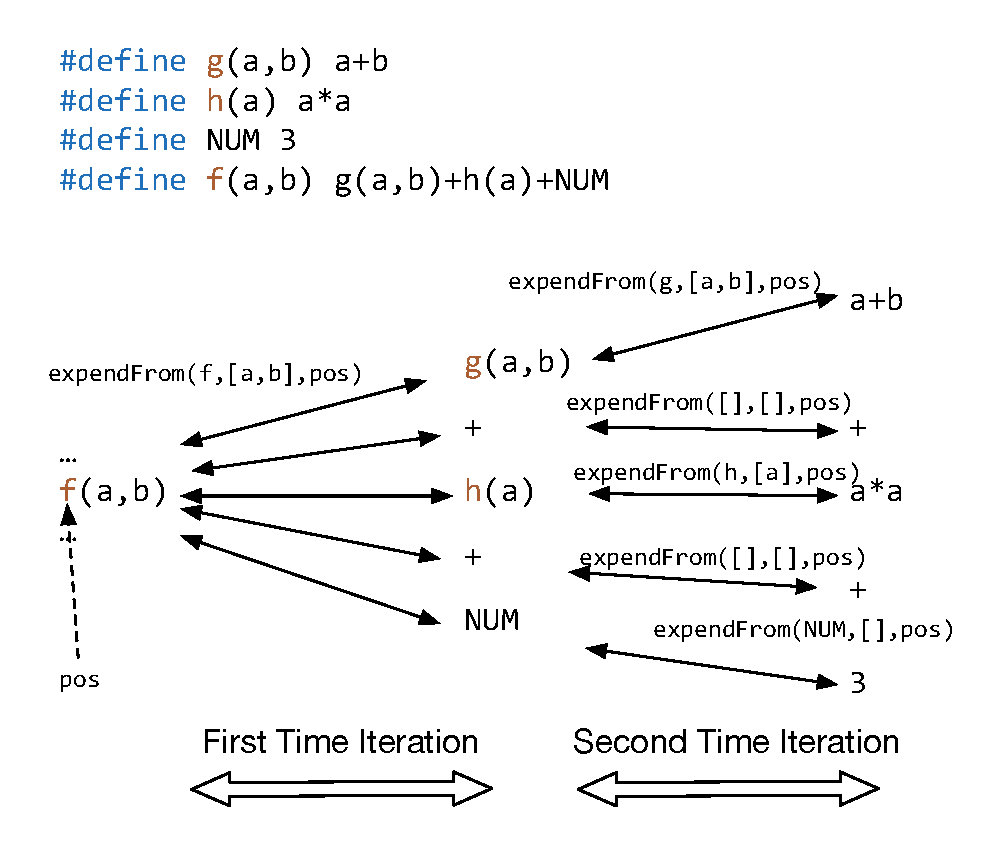
\includegraphics[width=9cm]{quick_example.eps}
\caption{MEDG of Quick Example.}
\end{figure}

Here is our pseudo code of Preprocessor $\mathtt{PP}$. 

\begin{algorithm}
    \caption{Preprocessor}
    \begin{algorithmic}[1] 
        \Require Original Code
        \Ensure Preprocessed Code with MEDG
        \Function{IterateOnce}{$ctx$}
        \EndFunction
            
    \end{algorithmic}
\end{algorithm}
\newpage

\section{Deal with Changes on Code with MEDG}
In this section, we will show how to deal with changes on preprocessded code and transform the changes back after we record macro call information with MEDG. We will first give out an example, then discuss the pesudo code for dealing with changes on code.

\begin{figure}[H]
\centering
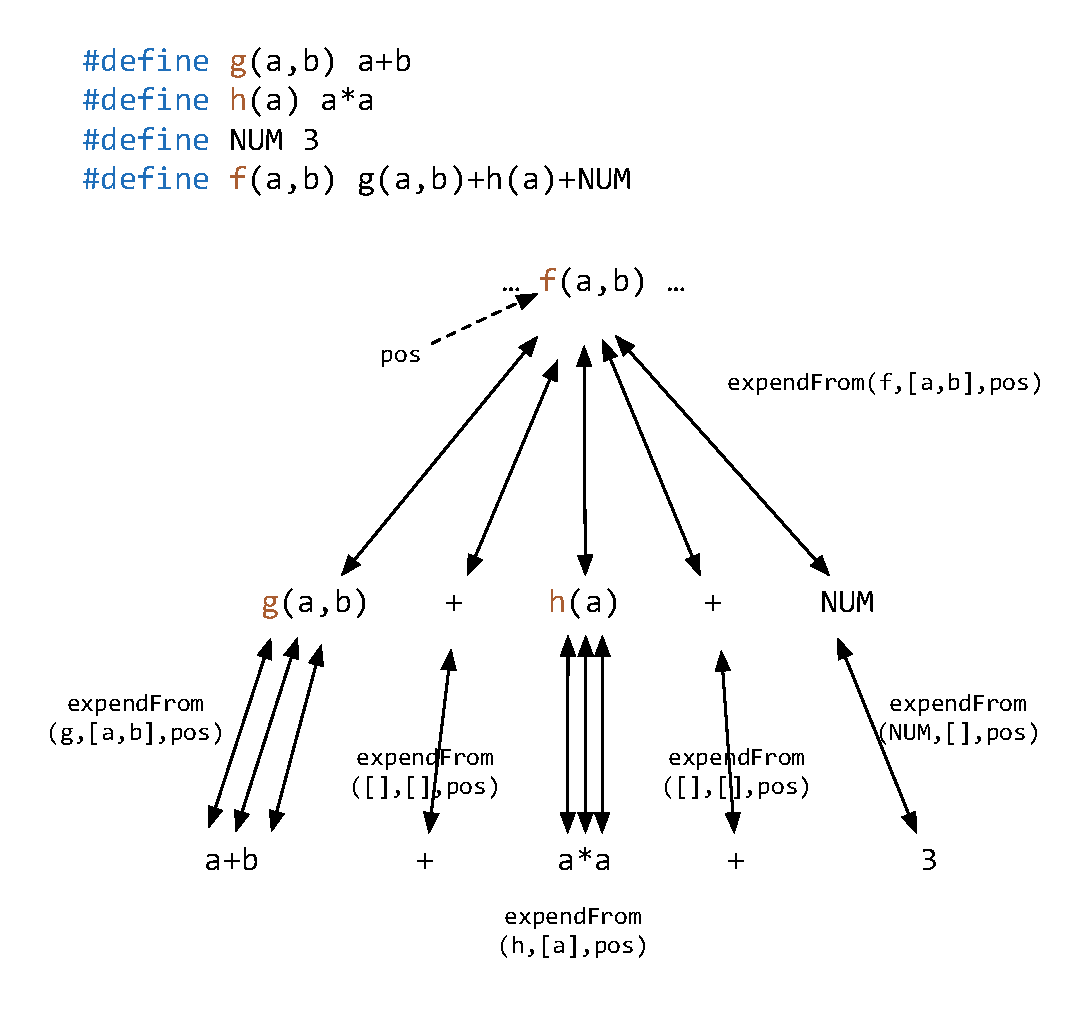
\includegraphics[width=9cm]{original.eps}
\caption{MEDG without Changes.}
\end{figure}

\begin{figure}[H]
\centering
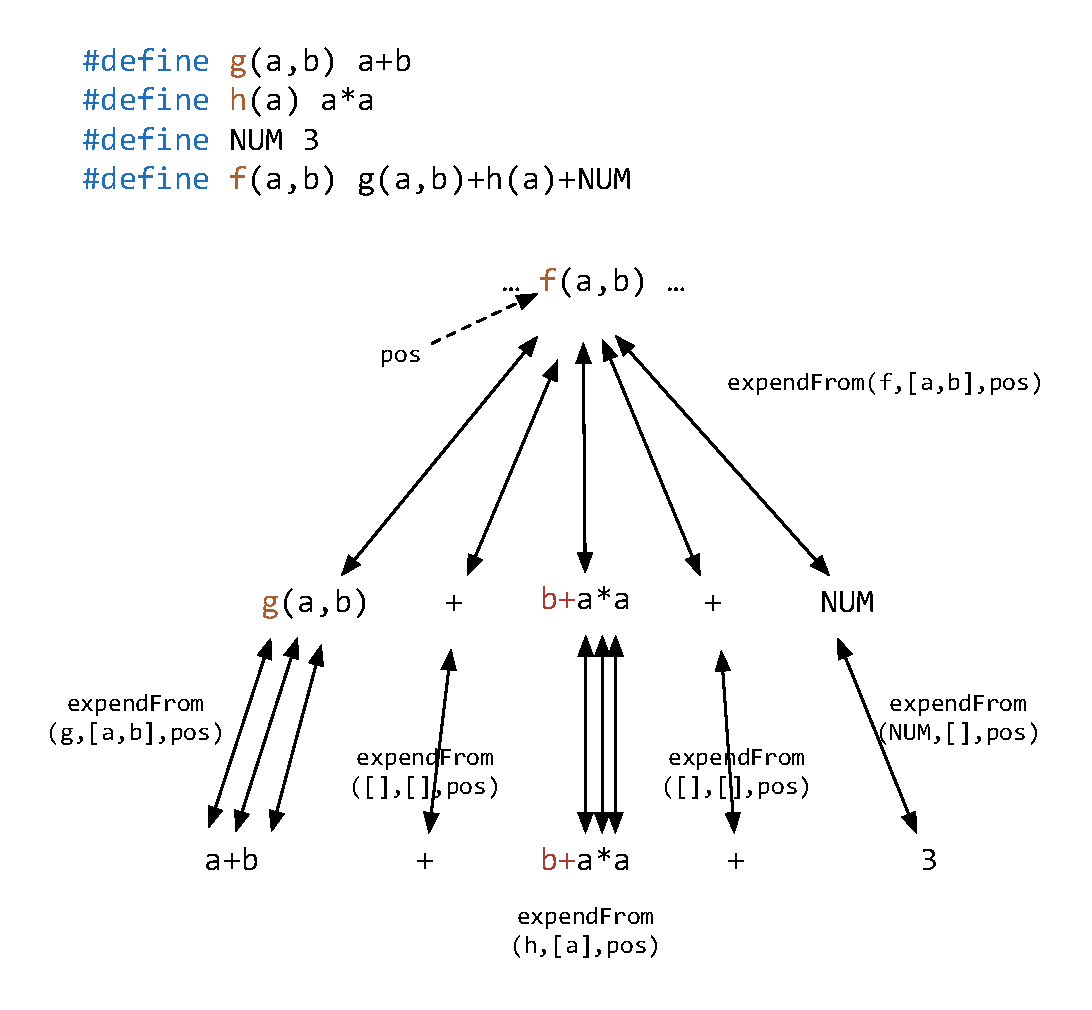
\includegraphics[width=9cm]{add_case.eps}
\caption{Adding Tokens to the Preprocessed Code.}
\end{figure}

\newpage
    \begin{algorithm}
        \caption{a}
        \begin{algorithmic}[1] 
            \Require a
            \Ensure a
            \Function {MergerSort}{$Array, left, right$}
                \State $result \gets 0$
                \If {$left < right$}
                    \State $middle \gets (left + right) / 2$
                    \State $result \gets result +$ \Call{MergerSort}{$Array, left, middle$}
                    \State $result \gets result +$ \Call{MergerSort}{$Array, middle, right$}
                    \State $result \gets result +$ \Call{Merger}{$Array,left,middle,right$}
                \EndIf
                \State \Return{$result$}
            \EndFunction
            \State
            \Function{Merger}{$Array, left, middle, right$}
                \State $i\gets left$
                \State $j\gets middle$
                \State $k\gets 0$
                \State $result \gets 0$
                \While{$i<middle$ \textbf{and} $j<right$}
                    \If{$Array[i]<Array[j]$}
                        \State $B[k++]\gets Array[i++]$
                    \Else
                        \State $B[k++] \gets Array[j++]$
                        \State $result \gets result + (middle - i)$
                    \EndIf
                \EndWhile
                \While{$i<middle$}
                    \State $B[k++] \gets Array[i++]$
                \EndWhile
                \While{$j<right$}
                    \State $B[k++] \gets Array[j++]$
                \EndWhile
                \For{$i = 0 \to k-1$}
                    \State $Array[left + i] \gets B[i]$
                \EndFor
                \State \Return{$result$}
            \EndFunction
        \end{algorithmic}
    \end{algorithm}
\end{document}